\section{De RNN's a Transformers}

Las \textbf{Redes Neuronales Recurrentes} o \textbf{RNN} (por sus siglas en Inglés) datan del año
1986, basadas en el trabajo de Rumelhart \cite{Rumelhart}. Este tipo de redes están especializadas
en el procesamiento de datos que contienen información temporal, mejorando los resultados obtenidos
por otros tipos de redes como \textit{Redes FeedForward} o \textit{Redes Convolucionales}.

La principal idea detrás de estos modelos de red es el concepto de \textit{Parameter Sharing}.
Con \textit{Parameter Sharing} un modelo un modelo puede generalizar mejor cuando la información
que esta contenida en diferentes partes de una secuencia. Así, el modelo no necesita aprender
independientemente todas las reglas que forman la secuencias, sino que ahora, la salida para cada
elemento en el tiempo esta determinada por la salida del elemento anterior. Resultando en una
recurrencia con las mismas reglas de actualización aplicadas a cada elemento en el tiempo.
La ecuación \ref{eq:rnn} representa este proceso; $h^{(t)}$ es el estado de la recurrencia aplicada
por alguna función $f$ a un elemento $x^{(t)}t$ de la secuencia $x$ en el tiempo, $t$ y $\theta$ son
los parámetros compartidos.

\begin{equation}
    h^{(t)} = f(h^{(t-1)}, x^{(t)}; \theta)
\end{equation}
\label{eq:rnn}

En una \textit{RNN} vista como un \textit{gráfo computacional dirigído y acíclico}, cada nodo
representa un estado en la recurrencia y procesa la información de la secuencia $x$ con los mismos
parámetros $\theta$ en cada paso, observe la figura \ref{fig:rnn_cg}.

\begin{figure}[h!]
\centering
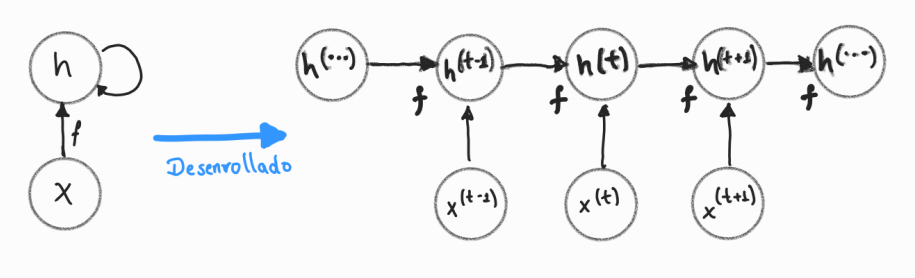
\includegraphics[width=.8\textwidth]{Chapters/1. Transformer/Figures/rnn/rnn_cgraph.png}
\caption[RNN - Grafo Computacional]{Grafo computacional generado por una \textit{RNN} al "desenrrollar" la
recurrencia. Usando los parámetros compartidos en cada nodo, con cada elemento $x^{(t)}$ de la
secuencia genera un nuevo estado oculto $h^{(t)}$ para retroalimentar nuevamente la entrada del
siguiente nodo.}
\label{fig:rnn_cg}
\end{figure}

Existen diversas formas como construir \textit{Redes neuronales Recurrentes}, pueden producir una
salida en cada paso de tiempo o tener solo una al final de la recurrencia  y también pueden tener
conexiones entre unidades ocultas. La manera más común de implementar una \textit{RNN} está ilustrada en la
figura \ref{fig:rnn_cfga}. En eta figura, cada etapa de la recurrencia es retroalimentada por la
activación del estado oculto previo. Así, $h^{(t)}$ contiene información codificada de elementos
previos de la secuencia que puede ser usada en el futuro para obtener una salida $O^{(t+1)}$. En la
figura \ref{fig:rnn_cfgb} se
cambia la retroalimentación de $h^{(t)}$ por $O^{(t)}$. Nótese que en este caso, la red es entrenada
para obtener un valor en específico $O^{(t)}$ lo que provocaría que gran parte de la información de
los estados ocultos pasados $h^{(t-1)}, h^{(t-2)}, ...$ no se transmita. En el esquema anterior
\ref{fig:rnn_cfga} la red es entrenada para decidir que información debe transmitir en el futuro a través
de los estados ocultos, en cambio, en la figura \ref{fig:rnn_cfgb} cada estado esta conectado con el
pasado a través de la predicción del paso anterior, perdiendo así gran parte de la información
codificada en los estados ocultos, a menos que la salida $O^{(t-1)}$ sea lo suficientemente rica y
esté en altas dimensiones.

% \begin{figure}[h!]
% \centering
% 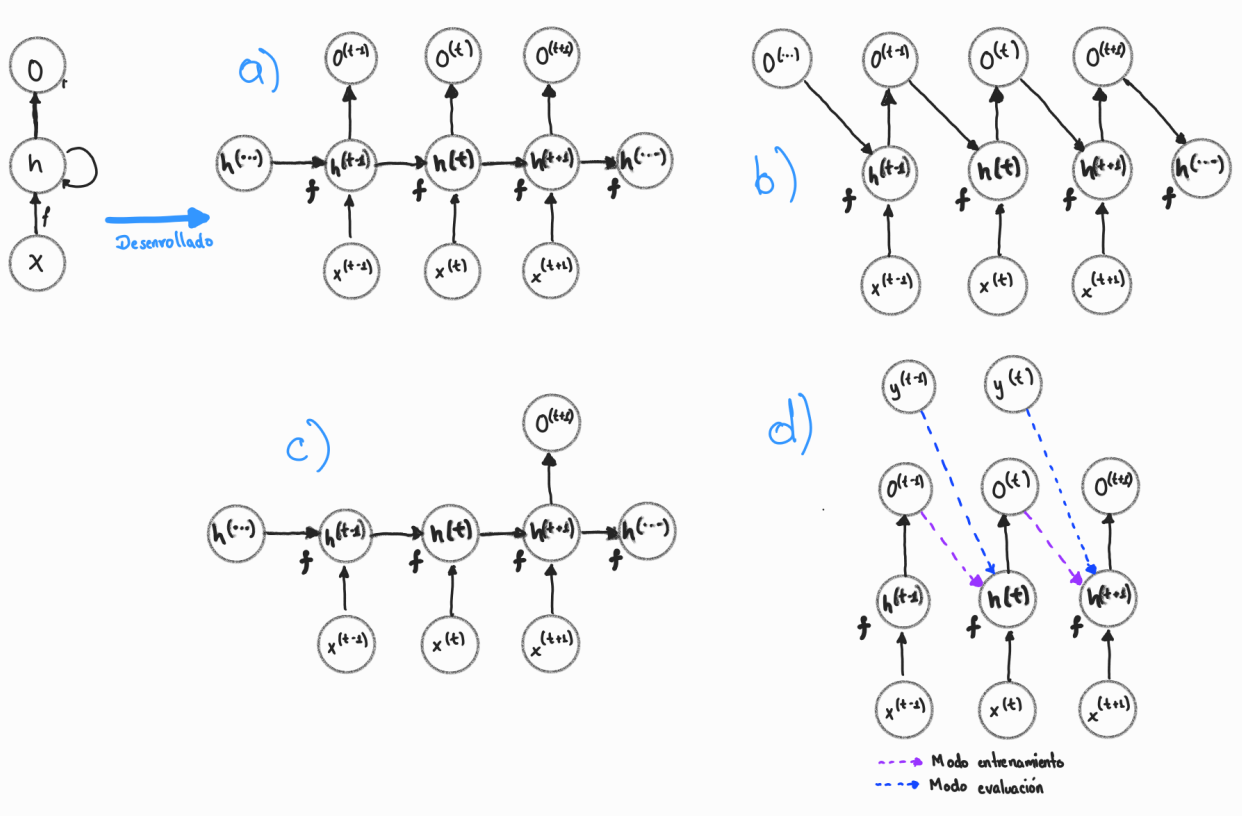
\includegraphics[width=.8\textwidth]{Chapters/1. Transformer/Figures/rnn/rnn_cfg.png}
% \caption[RNN - CFG]{Distintos tipos de RNNs. \textbf{a)} Las activaciones de las capas ocultas $h^{(t)}$
% alimentan al nodo siguiente, cada etapa de la recurrencia genera una salida $O^{(t)}$ \textbf{b)}
% Cada nodo es alimentado por las salidas de cada estado oculto $O^{(t)}$. \textbf{c)} Al final de la
% recurrencia solo tiene una salida $O^{(T)}$, puede ser usada para resumir/predecir un valor de una
% secuencia. \textbf{d)} Teacher Forcing. En modo de entrenamiento cada nodo en el tiempo $t$ es
% retroalimentado por la salida correcta $y^{(t-1)}$, en modo evaluación es retroalimentado por las
% salidas del modelo $O^{(t-1)}$}
% \label{fig:rnn_cfg}
% \end{figure}

\begin{figure}[h!]
    \centering
    \begin{subfigure}[b]{0.49\textwidth}
        \centering
        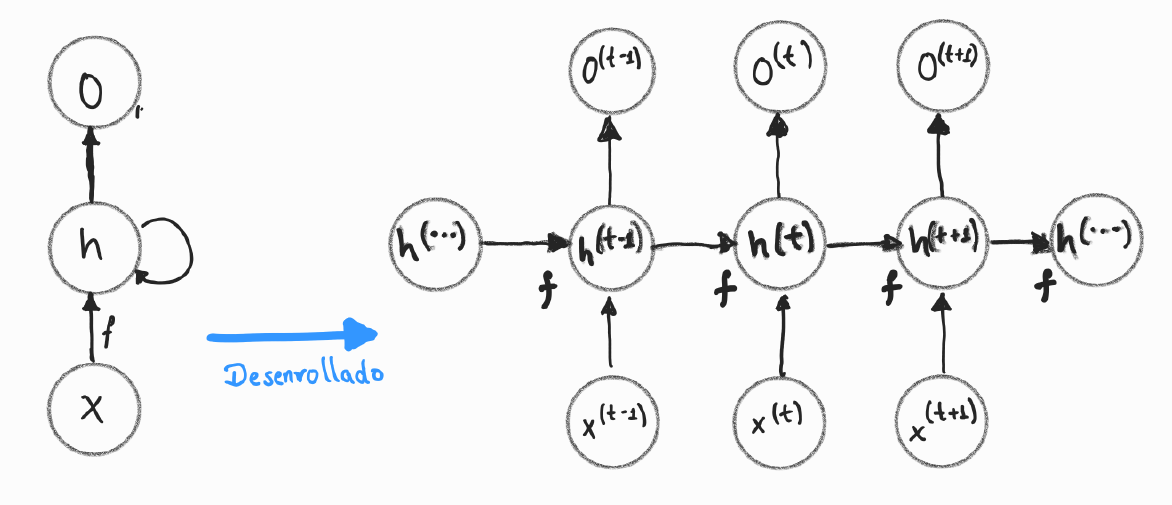
\includegraphics[width=\textwidth]{Chapters/1. Transformer/Figures/rnn/rnn_cfga.png}
        \caption{Las activaciones de las capas ocultas $h^{(t)}$
        alimentan al nodo siguiente, cada etapa de la recurrencia genera una salida $O^{(t)}$.}
        \label{fig:rnn_cfga}
    \end{subfigure}
    \hfill
    \begin{subfigure}[b]{0.4\textwidth}
        \centering
        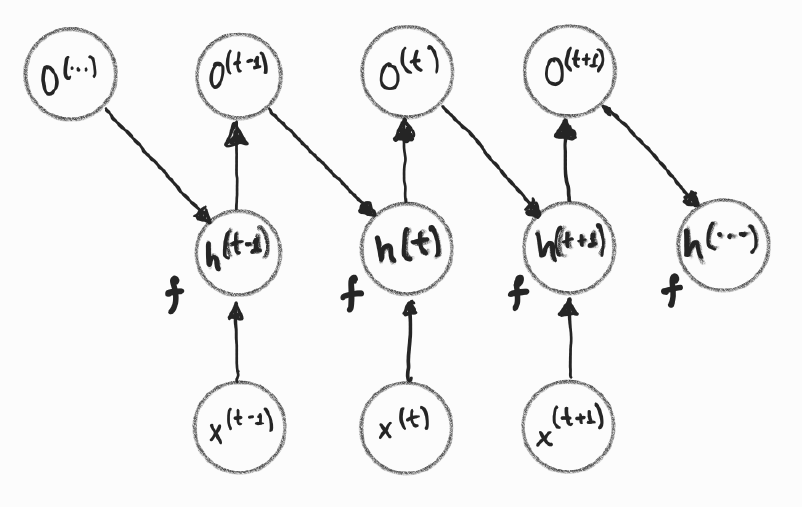
\includegraphics[width=\textwidth]{Chapters/1. Transformer/Figures/rnn/rnn_cfgb.png}
        \caption{Cada nodo es alimentado por las salidas de cada estado oculto $O^{(t)}$.}
        \label{fig:rnn_cfgb}
    \end{subfigure}

    \begin{subfigure}[b]{0.4\textwidth}
        \centering
        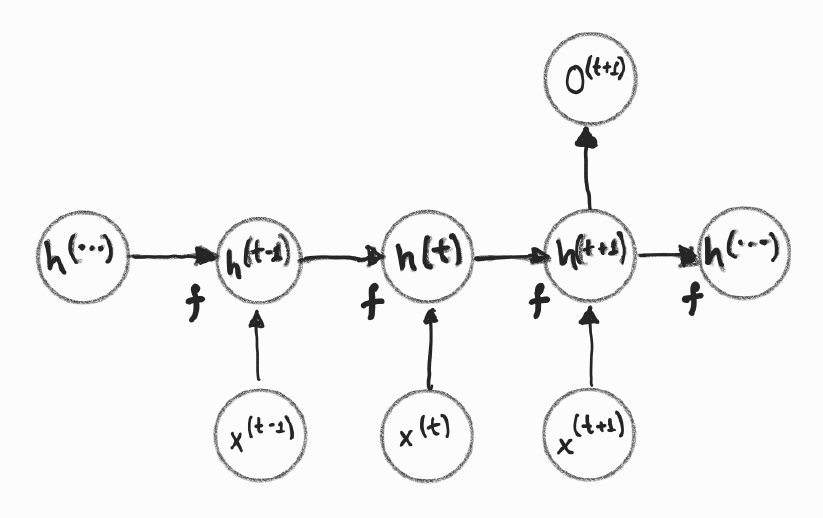
\includegraphics[height=0.63\textwidth]{Chapters/1. Transformer/Figures/rnn/rnn_cfgc.png}
        \caption{Al final de la recurrencia solo tiene una salida $O^{(T)}$, puede ser usada para
        resumir/predecir un valor de una secuencia.}
        \label{fig:rnn_cfgc}
    \end{subfigure}
    \hfill
    \begin{subfigure}[b]{0.49\textwidth}
        \centering
        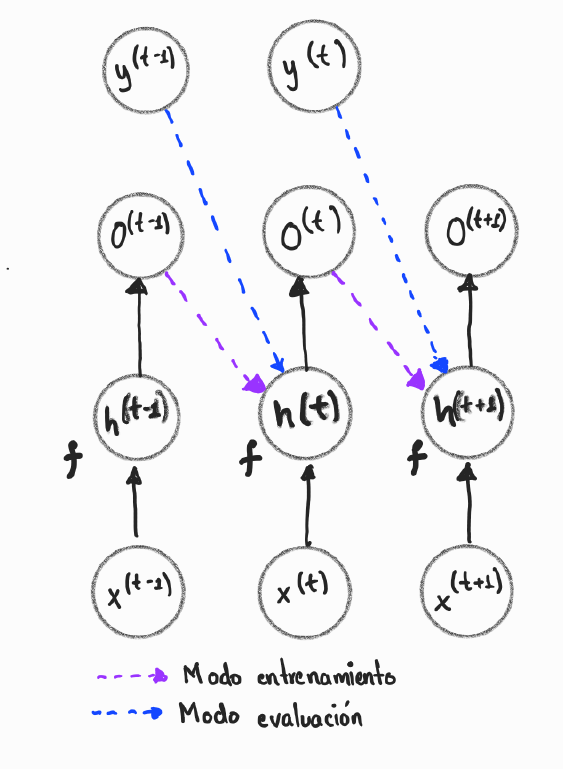
\includegraphics[height=0.6\textwidth]{Chapters/1. Transformer/Figures/rnn/rnn_cfgd.png}
        \caption{Teacher Forcing. En modo de entrenamiento cada nodo en el tiempo $t$ es
        retroalimentado por la salida correcta $y^{(t-1)}$, en modo evaluación es retroalimentado por las
        salidas del modelo $O^{(t-1)}$.}
        \label{fig:rnn_cfgd}
    \end{subfigure}

    \caption[RNN - CFG]{Distintos tipos de RNNs.}
    \label{fig:three graphs}
\end{figure}


Por otro lado, la \textit{RNN} representada en la figura \ref{fig:rnn_cfgc} tiene una sola salida al
final de la recurrencia.
Al contrario de las anteriores, este tipo de redes pueden ser usadas para resumir
información contenida en la secuencia para finalmente predecir un único valor final.
El \textit{Análisis de Sentimiento} en textos es una tarea común que puede ser representada con este esquema
de red. En la figura \ref{fig:rnn_cfgd} vemos un modelo de \textit{RNN} entrenado mediante el proceso de
Teacher Forcing; durante el entrenamiento la red es retroalimentada con las salidas
esperadas del modelo $y^{(t)}$ en el tiempo $t+1$. La ventaja de esta red es que al ser eliminadas
las conexiones entre estados ocultos, las funciones de pérdida basadas en comparar la predicción en
el tiempo $t$ con el valor objetivo $y^{(t)}$ pueden ser desacopladas. Por tanto, el entrenamiento
puede ser paralelizado al calcular el gradiente para cada tiempo $t$ por separado, puesto que ya
tenemos el valor ideal para esta salida.

Finalmente, en la figura \ref{fig:rnn_cfge} la Red Neuronal Recurrente es modificada para esta vez
no procesar una secuencia, sino que, procesa un solo vector en cada paso. El estado oculto
previo $h^{(t-1)}$ retroalimenta al siguiente paso $t$ así como la predicción esperada $y^{(t)}$ que
también es usada para calcular la función de costo del paso anterior $L^{(t-1)}$. Esta estructura de
red puede ser usada en tareas como Image Captioning, en donde la entrada es una imagen y la salida
una secuencia de palabras que describen esta misma.

\begin{figure}[h!]
\centering
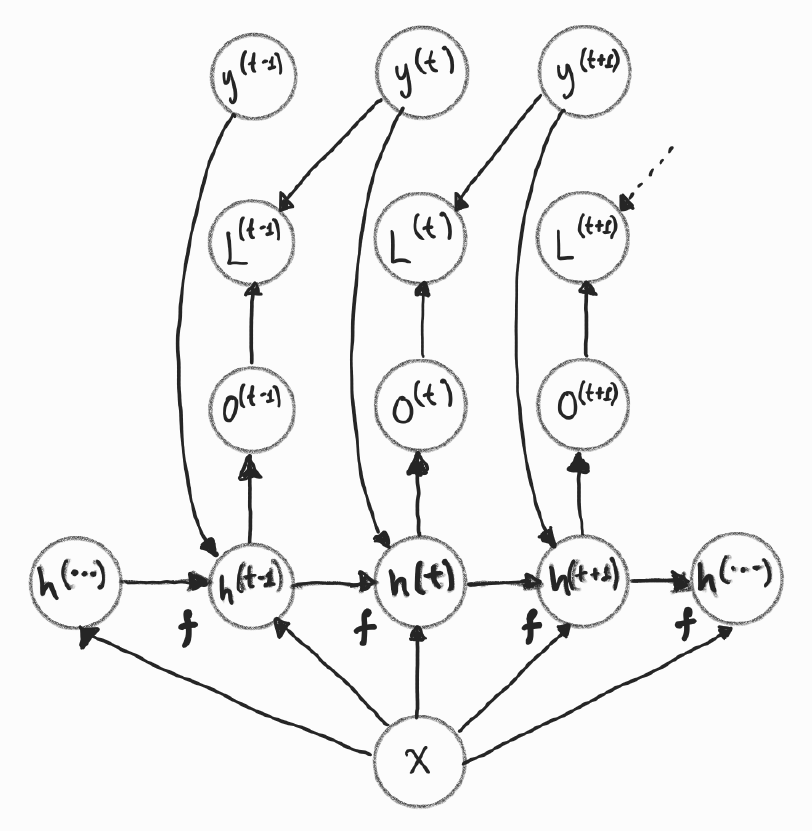
\includegraphics[width=.4\textwidth]{Chapters/1. Transformer/Figures/rnn/rnn_cfge.png}
\caption[RNN - Image Captioning]{Modelo usado para tareas de \textit{Image Captioning}, la entrada es una
sola imagen y la red predice una secuencia de palabras que describen dicha imagen La salida esperada
$y^{(t)}$ sirve como objetivo para la función de costo del paso anterior y como entrada en cada paso.}
\label{fig:rnn_cfge}
\end{figure}


Si bien, los modelos ejemplificados anteriormente son construidos de forma \textit{causal}, es
decir, la secuencia es procesada en un solo sentido, estos pueden ser modificados fácilmente para
que las secuencias sean procesadas en ambas direcciones, a lo que llamamos \textbf{Redes Neuronales
Recurrentes Bidireccionales}.



- Celdas de memoria LSTM GRU

- Attention mechanism
- Mencionar parallización y backpropragation trougth the time

- Problema de RNN
Vanising gradient
https://www.iro.umontreal.ca/~lisa/pointeurs/ieeetrnn94.pdf
https://arxiv.org/pdf/1211.5063.pdf





\section{El modelo Transformer}

A finales del año 2017 se presentó un nuevo modelo que vino a revolucionar el área de Procesamiento
de Lenguaje Natural, El Transformer \cite{Vaswani}. Una de sus principales características es la
capacidad de procesar la información de alguna secuencia de forma paralela, caso contrario a las
Redes Neuronales Recurrentes, donde la información se procesa recurrentemente. Gracias a ello
la capacidad de \textit{recuerdo} no se ve afectado por el problema de \textit{El
desvanecimiento del Gradiente} cuando se trabaja con secuencias bastante largas.
